% document
\documentclass[11pt]{article}
\usepackage[letterpaper, portrait, margin=0.75in]{geometry}
\usepackage{setspace}
\usepackage{color}

% text
\usepackage[utf8]{inputenc}
\setlength\parindent{0pt}
\setlength{\parskip}{1em}
\usepackage{enumitem}
\renewcommand{\familydefault}{\sfdefault}
\newcommand{\RomanNumeral}[1]{\textrm{\uppercase\expandafter{\romannumeral #1\relax}}}

% math
\usepackage{amssymb}
\usepackage{amsmath}
\usepackage[cm]{sfmath}
\usepackage{commath}
\usepackage{multirow}
\DeclareMathAlphabet{\mathpzc}{OT1}{pzc}{m}{it}

% graphics
\usepackage{graphics}
\usepackage{graphicx}
\usepackage{epsfig}
\usepackage{epstopdf}
\usepackage{xpatch}
\usepackage{pdfpages}

% "S" prefix
\renewcommand{\theequation}{S\arabic{equation}}
\renewcommand{\thefigure}{S\arabic{figure}}
\renewcommand{\thetable}{S\arabic{table}}

% each section begins new page
\let\stdsection\section
\renewcommand\section{\clearpage\stdsection}

% hyperref
\usepackage{hyperref}
\hypersetup{
	colorlinks,
	bookmarksopen,
	bookmarksnumbered,
	hidelinks,
}
\usepackage[all]{hypcap}  % helps hyperref work properly

% bibliography
\usepackage[numbers]{natbib}

\begin{document}
\setcounter{page}{1}
\renewcommand{\thepage}{S\arabic{page}}

\begin{center}
	\LARGE

        Supporting Information

        Open Source Photoreactor

	\normalsize

	\textit{Philip Lampkin, Blaise J. Thompson, and Samuel H. Gellman*}

	Department of Chemistry, University of Wisconsin--Madison\\
	1101 University Ave., Madison, Wisconsin 53706
\end{center}

\vspace{\fill}

*Corresponding Author \\
\hspace*{2ex} email: gellman@chem.wisc.edu \\

\pagebreak
\renewcommand{\baselinestretch}{0.75}\normalsize
\tableofcontents
\renewcommand{\baselinestretch}{1.0}\normalsize
\pagebreak

\section{Introduction}

\section{Electronics}

\subsection{Analog}

\includepdf[landscape=true]{"../analog-driver/driver.pdf"}

\subsection{Digital}

\subsubsection{Driver}

\includepdf[landscape=true]{"../digital-driver/driver.pdf"}

\subsubsection{Controller}

\section{Mechanical Construction}

\subsection{Base}

\subsubsection{LED and Heatsink}

TODO: LED PCB part number

TODO: heatsink part number

Tap the heatsink.

TODO: heatsink compoud

Install with wires facing towards printed hole

Use 4-40 1/4''.

\subsubsection{Fan}

TODO: fan part number

Noctua NF-A12x15 PWM

pins:
blue: PWM (5 V)
yellow: +12 V
black: ground

Use 4-40 3/4'' into captured nuts

\section{Efficacy}

\end{document}
